
%(BEGIN_QUESTION)
% Copyright 2009, Tony R. Kuphaldt, released under the Creative Commons Attribution License (v 1.0)
% This means you may do almost anything with this work of mine, so long as you give me proper credit

Bestem alle handlinger som vil gi en {\it økt} produkttemperatur i ``hot product''-røret (når det forlater varmeveksleren), forutsatt bruk av mettet damp (dvs. damp ved sin koke-/kondenseringstemperatur) som oppvarmingsmedium:

$$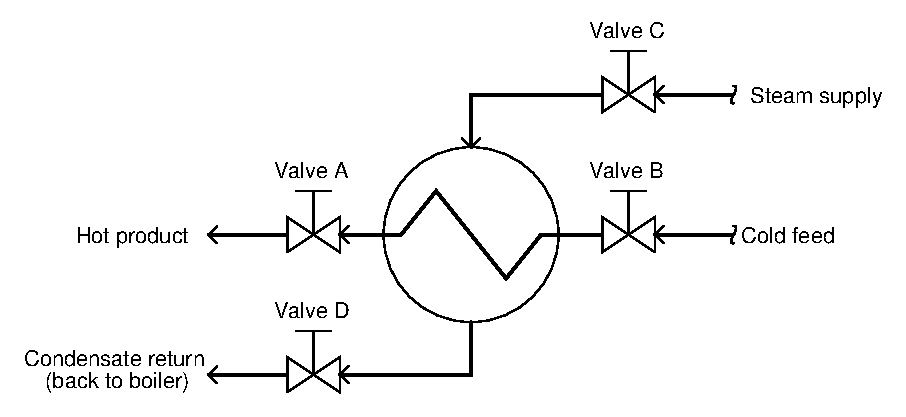
\includegraphics[width=15.5cm]{i00015x01.eps}$$

Angi om hver mulig handling i listen vil gi økt produkttemperatur eller ikke, ved å krysse av i tabellen.  Anta at alle ventiler struper (hverken helt åpne eller helt lukket, men hver arbeider for å begrense strømning), og at ordene ``åpne'' og ``lukke'' refererer til små endringer, ikke ekstrem posisjon (dvs. åpne eller lukke litt, ikke {\it fullt} åpne eller {\it fullt} lukke):

% No blank lines allowed between lines of an \halign structure!
% I use comments (%) instead, so that TeX doesn't choke.

$$\vbox{\offinterlineskip
\halign{\strut
\vrule \quad\hfil # \ \hfil & 
\vrule \quad\hfil # \ \hfil & 
\vrule \quad\hfil # \ \hfil \vrule \cr
\noalign{\hrule}
%
% First row
{\bf Handling} & {\bf Vil virke} & {\bf Vil ikke virke} \cr
%
\noalign{\hrule}
%
% Another row
Åpne ventil A &  & \cr
%
\noalign{\hrule}
%
% Another row
Lukke ventil A &  & \cr
%
\noalign{\hrule}
%
% Another row
Åpne ventil B &  & \cr
%
\noalign{\hrule}
%
% Another row
Lukke ventil B &  & \cr
%
\noalign{\hrule}
%
% Another row
Øke damptilførselstrykket &  & \cr
%
\noalign{\hrule}
%
% Another row
Redusere damptilførselstrykket &  & \cr
%
\noalign{\hrule}
%
% Another row
Øke innkommende medietemperatur &  & \cr
%
\noalign{\hrule}
%
% Another row
Åpne ventil C &  & \cr
%
\noalign{\hrule}
%
% Another row
Lukke ventil C &  & \cr
%
\noalign{\hrule}
} % End of \halign 
}$$ % End of \vbox


\vfil 

\underbar{file i00015}
\eject
%(END_QUESTION)





%(BEGIN_ANSWER)

Dette er et vurdert spørsmål -- ingen svar eller hint gis!

%(END_ANSWER)





%(BEGIN_NOTES)

Et viktig prinsipp for enhver varmeveksler kan formuleres slik: {\it hvis væske ``A'' varmer væske ``B'', så kjøler væske ``B'' væske ``A''.}  I dette eksemplet brukes damp som oppvarmingsmedium for en ukjent produktvæske.  Dampen varmer produktet, mens produktet kjøler dampen.

\vskip 10pt

Enhver endring i dampstrøm med gitt produktstrøm vil direkte påvirke produkttemperaturen ut, og også kondensattemperaturen.  Den direkte påvirkningen av dampstrøm på produkttemperaturen er enkel å se: mer eller mindre varm damp inn i veksleren endrer mengden varme tilført produktet, og dermed produkttemperaturen.  Den direkte påvirkningen på kondensattemperaturen er lettest å se fra kjøleperspektivet: dampstrømmen påvirker hvor lang {\it tid} hver dampmolekyl tilbringer i veksleren mens den kjøles av produktet.

\vskip 10pt

Enhver endring i produktstrøm med gitt dampstrøm vil omvendt påvirke produkttemperaturen ut, og også omvendt påvirke kondensattemperaturen.  Den omvendte påvirkningen av produktstrøm på produkttemperaturen ut skyldes tiden hvert produktmolekyl tilbringer i veksleren og blir varmet av dampen.  Den omvendte påvirkningen på kondensattemperaturen skyldes endringen i hvor mye produktet kjøler dampen.


% No blank lines allowed between lines of an \halign structure!
% I use comments (%) instead, so that TeX doesn't choke.

$$\vbox{\offinterlineskip
\halign{\strut
\vrule \quad\hfil # \ \hfil & 
\vrule \quad\hfil # \ \hfil & 
\vrule \quad\hfil # \ \hfil \vrule \cr
\noalign{\hrule}
%
% First row
{\bf Handling} & {\bf Vil virke} & {\bf Vil ikke virke} \cr
%
\noalign{\hrule}
%
% Another row
Åpne ventil A &  & $\surd$ \cr
%
\noalign{\hrule}
%
% Another row
Lukke ventil A & $\surd$  & \cr
%
\noalign{\hrule}
%
% Another row
Åpne ventil B &  & $\surd$ \cr
%
\noalign{\hrule}
%
% Another row
Lukke ventil B & $\surd$  & \cr
%
\noalign{\hrule}
%
% Another row
Øke damptilførselstrykket & $\surd$  & \cr
%
\noalign{\hrule}
%
% Another row
Redusere damptilførselstrykket &  & $\surd$ \cr
%
\noalign{\hrule}
%
% Another row
Øke innkommende medietemperatur & $\surd$  & \cr
%
\noalign{\hrule}
%
% Another row
Åpne ventil C & $\surd$  & \cr
%
\noalign{\hrule}
%
% Another row
Lukke ventil C &  & $\surd$ \cr
%
\noalign{\hrule}
} % End of \halign 
}$$ % End of \vbox


%INDEX% Physics, temperature: heat exchangers
%INDEX% Process: heat exchanger temperature/flow control (generic)

%(END_NOTES)
